% ===================================================================
%  Глава 2. Проектирование веб-приложения
%  Типы колонок M{} и L{} объявлены в paper.tex
%  \include автоматически добавляет \newpage перед главой
% ===================================================================

\phantomsection
\section*{Глава 2. Проектирование веб-приложения}
\addcontentsline{toc}{section}{Глава 2. Проектирование веб-приложения}
\stepcounter{section}

% -------------------------------------------------------------------
\subsection{Анализ целевой аудитории}
\label{subsec:audience}
% -------------------------------------------------------------------

Разрабатываемое приложение RestaurantBook предназначено для автоматизации
процесса бронирования столиков в ресторане. Система ориентирована на две
основные группы пользователей: авторизованных пользователей и администраторов.
Такое разделение необходимо, поскольку пользовательские сценарии у этих
ролей различаются: авторизованный пользователь создаёт и отслеживает бронирование, а
администратор управляет данными, контролирует занятость столиков и
формирует отчёты.

\textbf{Авторизованный пользователь} --- посетитель ресторана, который после регистрации и входа в систему может заранее выбрать
дату, время, столик и получить подтверждение без телефонного звонка. Для
данной роли важны простая регистрация, просмотр меню, выбор свободного
столика, получение уведомлений в интерфейсе, email-уведомлений и
PDF-подтверждения бронирования.

\textbf{Администратор} --- сотрудник ресторана, который отвечает за
актуальность информации в системе. Он управляет столиками, меню,
бронированиями, статусами заявок, изображениями столиков и блюд, а также
получает отчёты о загруженности зала в форматах CSV и PDF.

Для описания целевой аудитории применён метод персонажей (Personas),
позволяющий формализовать потребности и типовые сценарии поведения
каждой роли~\cite{cooper_personas}. Разграничение прав доступа
реализуется на уровне аутентификации: обычный пользователь получает
доступ к пользовательским страницам, а администратор --- к панели
управления.

\begin{table}[H]
    \centering
    \caption{Характеристика целевой аудитории приложения}
    \label{tab:audience}
    \begin{tabular}{|L{45mm}|L{52mm}|L{50mm}|}
        \hline
        \centering\textbf{Роль} &
        \centering\textbf{Основные потребности} &
        \centering\arraybackslash\textbf{Ключевые функции системы} \\
        \hline
        Авторизованный пользователь &
        Забронировать столик, посмотреть меню, получить подтверждение и уведомления &
        Регистрация, вход, просмотр меню, проверка доступности столика, бронирование, внутренние и email-уведомления, PDF-подтверждение \\
        \hline
        Администратор &
        Управлять столиками, меню и бронированиями, контролировать загрузку зала &
        CRUD-интерфейс, загрузка изображений, изменение времени и статусов бронирований, отчёты CSV/PDF \\
        \hline
    \end{tabular}
\end{table}

% -------------------------------------------------------------------
\subsection{Описание функциональности приложения}
\label{subsec:functionality}
% -------------------------------------------------------------------

Функциональность системы была описана через пользовательские истории
(User Story). Такой формат позволяет зафиксировать требование с точки
зрения конкретной роли: кто выполняет действие, какую возможность он
получает и зачем она нужна~\cite{cohn_userstories}. В таблице
\ref{tab:user_stories} пользовательские истории сформулированы так,
чтобы показать основные сценарии работы пользователя и администратора
с системой бронирования.

\begingroup
\small
\setlength{\tabcolsep}{3pt}
\begin{longtable}{|L{48mm}|L{47mm}|L{43mm}|}
    \caption{Пользовательские истории системы RestaurantBook}
    \label{tab:user_stories} \\
    \hline
    \centering\textbf{Роль} &
    \centering\textbf{User Story} &
    \centering\arraybackslash\textbf{Результат} \\
    \hline
    \endfirsthead
    \hline
    \centering\textbf{Роль} &
    \centering\textbf{User Story} &
    \centering\arraybackslash\textbf{Результат} \\
    \hline
    \endhead
    Авторизованный пользователь & Я, как пользователь, хочу зарегистрироваться и войти в систему & Доступ к личным бронированиям и уведомлениям \\
    \hline
    Авторизованный пользователь & Я, как пользователь, хочу просмотреть меню ресторана & Возможность выбрать ресторанное предложение до бронирования \\
    \hline
    Авторизованный пользователь & Я, как пользователь, хочу проверить доступность столика на выбранные дату и время & Исключение выбора занятого столика \\
    \hline
    Авторизованный пользователь & Я, как пользователь, хочу создать бронирование с указанием времени начала и окончания & Фиксация резервации в системе \\
    \hline
    Авторизованный пользователь & Я, как пользователь, хочу получить уведомление в интерфейсе, email-сообщение и PDF-подтверждение после бронирования & Подтверждение факта бронирования и информирование пользователя \\
    \hline
    Администратор & Я, как администратор, хочу выполнять CRUD-операции со столиками & Актуальное состояние схемы зала \\
    \hline
    Администратор & Я, как администратор, хочу выполнять CRUD-операции с бронированиями & Возможность подтвердить, изменить или отменить заявку \\
    \hline
    Администратор & Я, как администратор, хочу загружать изображения столиков и блюд меню & Наглядное отображение данных в интерфейсе \\
    \hline
    Администратор & Я, как администратор, хочу экспортировать отчёты о занятости в CSV и PDF & Получение отчётности по загрузке столиков \\
    \hline
\end{longtable}
\endgroup

На рисунке~\ref{fig:use_case} представлена диаграмма вариантов
использования системы, построенная в нотации UML~\cite{uml_spec}. В
диаграмме отдельно показаны регистрация и вход, CRUD столиков и меню,
CRUD бронирований, загрузка изображений, проверка доступности столика,
управление временем бронирования, экспорт отчётов CSV/PDF, просмотр
уведомлений, получение email-уведомлений и генерация PDF-подтверждения.

\begin{figure}[H]
    \centering
    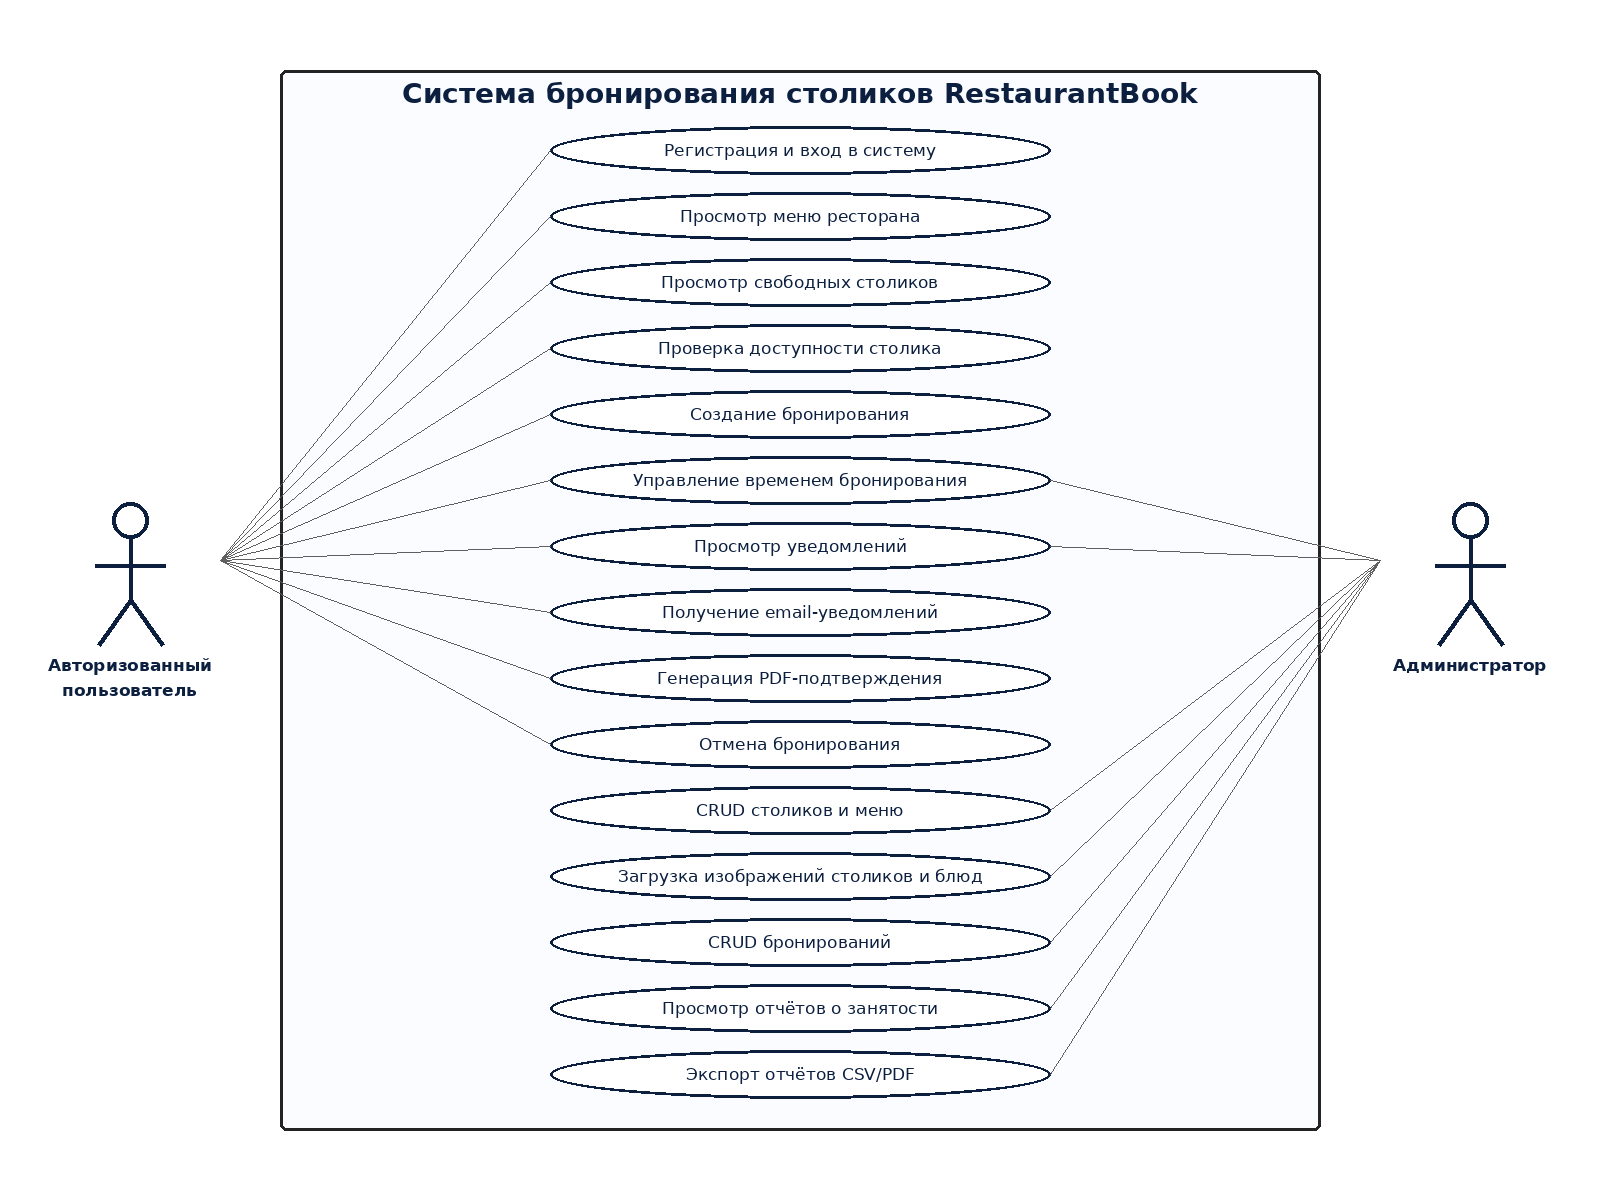
\includegraphics[width=0.95\textwidth]{use_case}
    \caption{Диаграмма вариантов использования системы}
    \label{fig:use_case}
\end{figure}

% -------------------------------------------------------------------
\subsection{Проектирование модели данных}
\label{subsec:db}
% -------------------------------------------------------------------

Для хранения данных приложения спроектирована реляционная модель. В неё
включены сущности пользователей, столиков, позиций меню, бронирований,
уведомлений и файлов подтверждений. Метод диаграмм сущность-связь
позволяет наглядно описать структуру данных и отношения между
сущностями~\cite{chen_er}. На рисунке~\ref{fig:er} представлена
ER-диаграмма. Связь между пользователем и бронированием вынесена в
обход центральной сущности, поэтому линия не проходит сквозь таблицы и
не ухудшает читаемость схемы.

\begin{figure}[H]
    \centering
    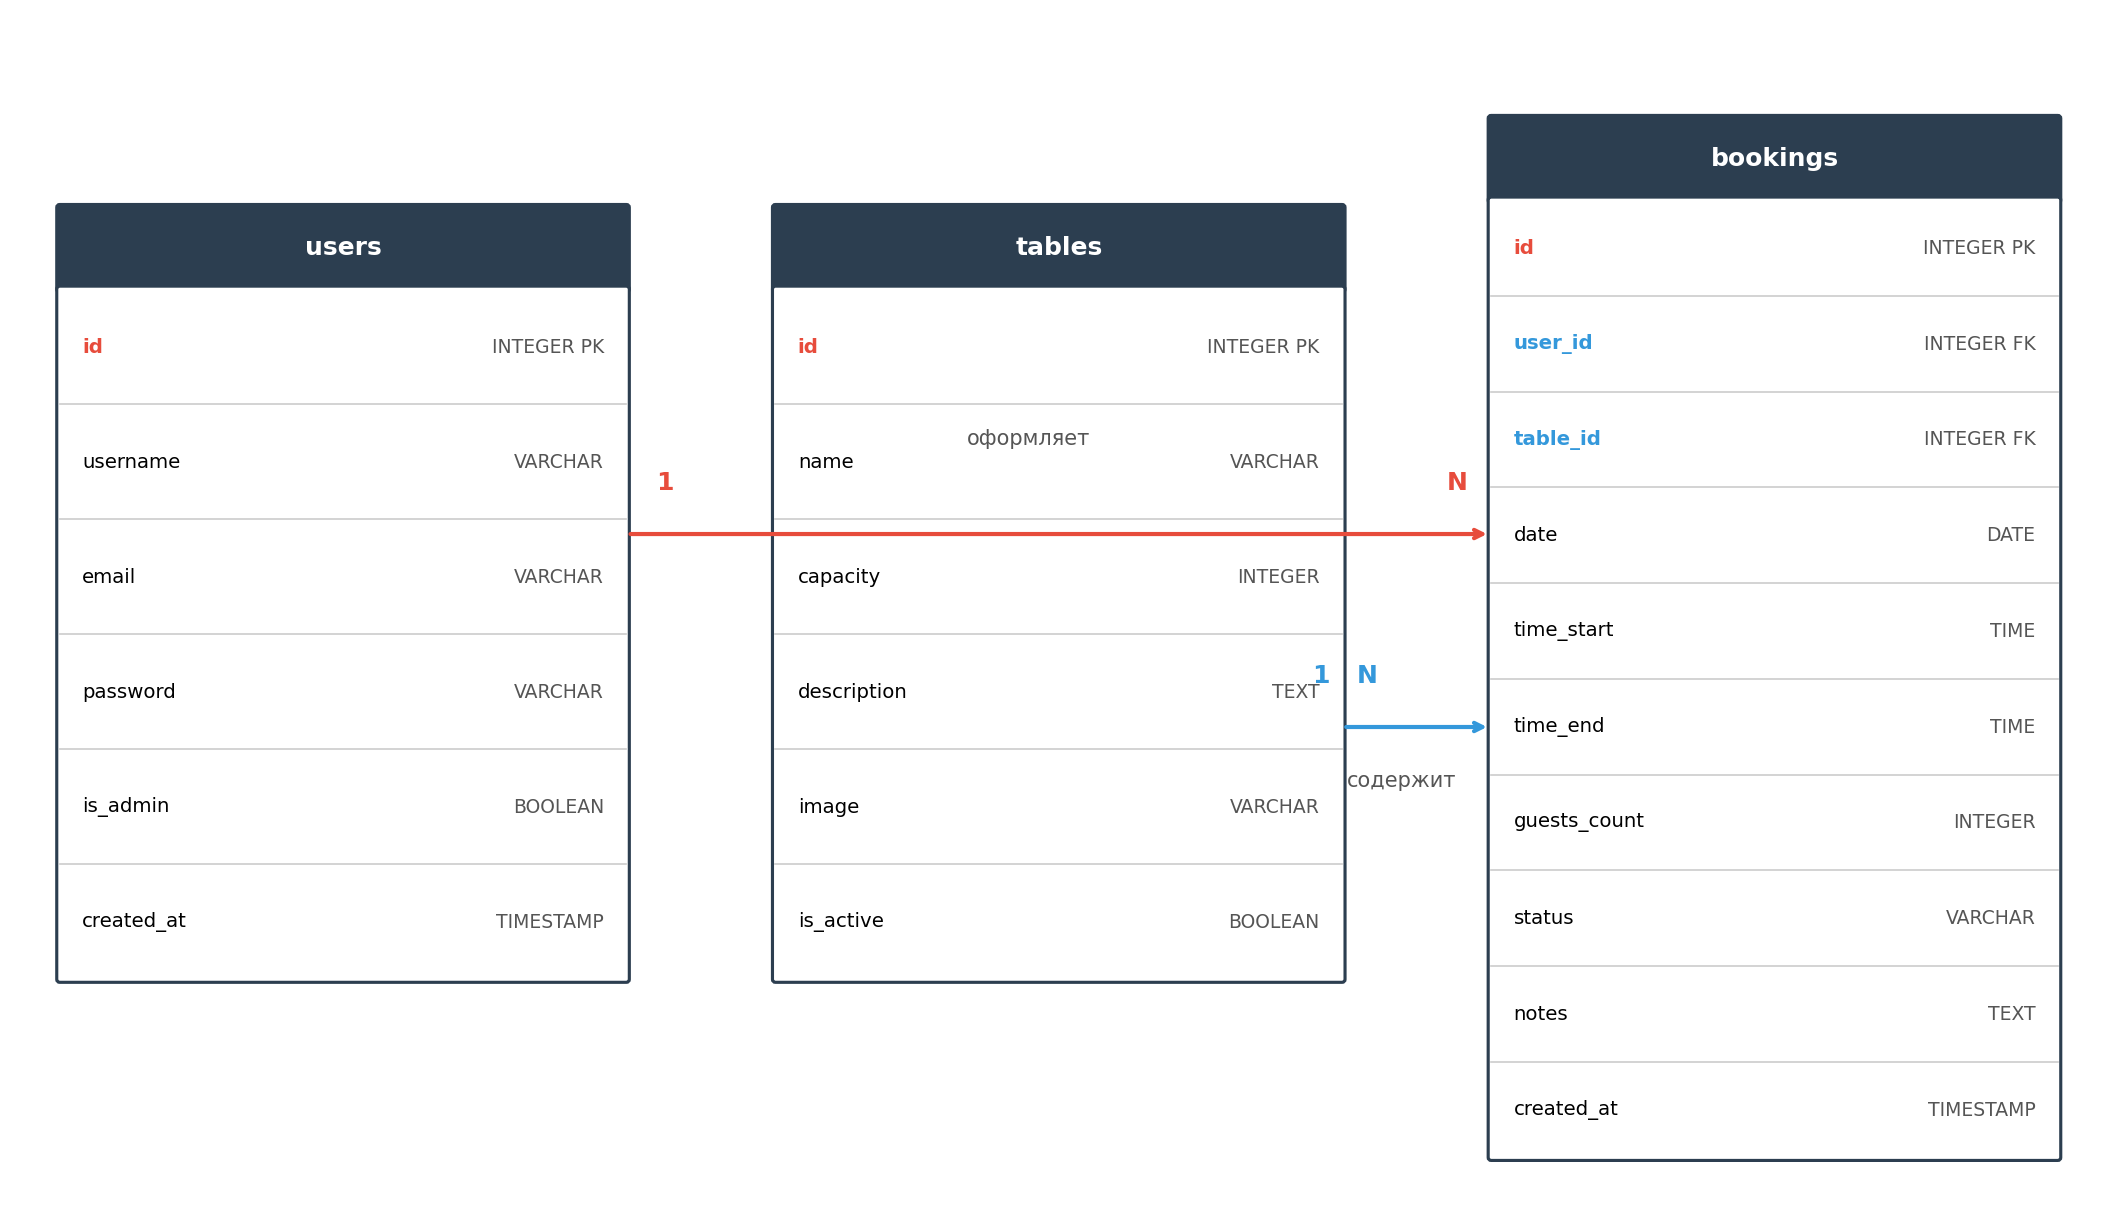
\includegraphics[width=0.95\textwidth]{er_diagram}
    \caption{ER-диаграмма модели данных}
    \label{fig:er}
\end{figure}

Сущность \texttt{users} используется для хранения данных пользователей:
логина, email, хэша пароля и роли. Сущности \texttt{tables},
\texttt{menu\_items} и \texttt{bookings} обеспечивают работу со столиками,
меню и бронированиями. Поля \texttt{image\_path} используются для хранения
путей к загруженным изображениям столиков и блюд меню. Сущность
\texttt{notifications} используется для хранения внутренних уведомлений и
сведений об email-рассылке. Поле \texttt{delivery\_channel} показывает канал
доставки уведомления: внутри сайта или на электронную почту. Поля
\texttt{email\_status} и \texttt{sent\_at} позволяют фиксировать результат и
время отправки письма. Сущность \texttt{booking\_files} используется для
файлов подтверждений бронирования. Она хранит сведения о сформированном
PDF-чеке: тип файла, путь к файлу и дату генерации. Благодаря отдельной
таблице можно хранить историю подтверждений и связывать каждый файл с
конкретным бронированием.

Структура таблицы пользователей приведена в таблице~\ref{tab:db_users}.

{\small
\begin{longtable}{|L{25mm}|L{22mm}|L{38mm}|L{55mm}|}
    \caption{Структура таблицы пользователей (users)}
    \label{tab:db_users} \\
    \hline
    \textbf{Поле} & \textbf{Тип} & \textbf{Ограничение} & \textbf{Описание} \\ \hline
    \endfirsthead
    \hline
    \textbf{Поле} & \textbf{Тип} & \textbf{Ограничение} & \textbf{Описание} \\ \hline
    \endhead
    id & INTEGER & PRIMARY KEY, AUTO & Уникальный идентификатор пользователя \\ \hline
    username & VARCHAR & NOT NULL, UNIQUE & Логин пользователя \\ \hline
    email & VARCHAR & NOT NULL, UNIQUE & Адрес электронной почты \\ \hline
    password\_hash & VARCHAR & NOT NULL & Хэш пароля пользователя \\ \hline
    role & VARCHAR & DEFAULT 'user' & Роль: пользователь или администратор \\ \hline
    created\_at & TIMESTAMP & DEFAULT NOW() & Дата и время регистрации \\ \hline
\end{longtable}
}

Структура таблицы столиков приведена в таблице~\ref{tab:db_tables}.

{\small
\begin{longtable}{|L{25mm}|L{22mm}|L{38mm}|L{55mm}|}
    \caption{Структура таблицы столиков (tables)}
    \label{tab:db_tables} \\
    \hline
    \textbf{Поле} & \textbf{Тип} & \textbf{Ограничение} & \textbf{Описание} \\ \hline
    \endfirsthead
    \hline
    \textbf{Поле} & \textbf{Тип} & \textbf{Ограничение} & \textbf{Описание} \\ \hline
    \endhead
    id & INTEGER & PRIMARY KEY, AUTO & Уникальный идентификатор столика \\ \hline
    name & VARCHAR & NOT NULL & Название или номер столика \\ \hline
    capacity & INTEGER & NOT NULL & Максимальное количество гостей \\ \hline
    description & TEXT & NULL & Описание расположения и особенностей \\ \hline
    image\_path & VARCHAR & NULL & Путь к фотографии столика \\ \hline
    is\_active & BOOLEAN & DEFAULT TRUE & Доступность столика для бронирования \\ \hline
\end{longtable}
}

Структура таблицы меню приведена в таблице~\ref{tab:db_menu}.

{\small
\begin{longtable}{|L{25mm}|L{22mm}|L{38mm}|L{55mm}|}
    \caption{Структура таблицы меню (menu\_items)}
    \label{tab:db_menu} \\
    \hline
    \textbf{Поле} & \textbf{Тип} & \textbf{Ограничение} & \textbf{Описание} \\ \hline
    \endfirsthead
    \hline
    \textbf{Поле} & \textbf{Тип} & \textbf{Ограничение} & \textbf{Описание} \\ \hline
    \endhead
    id & INTEGER & PRIMARY KEY, AUTO & Уникальный идентификатор блюда \\ \hline
    name & VARCHAR & NOT NULL & Название блюда \\ \hline
    category & VARCHAR & NOT NULL & Категория меню \\ \hline
    description & TEXT & NULL & Описание блюда \\ \hline
    price & DECIMAL & NOT NULL & Стоимость позиции \\ \hline
    image\_path & VARCHAR & NULL & Путь к изображению блюда \\ \hline
    is\_active & BOOLEAN & DEFAULT TRUE & Отображение позиции в меню \\ \hline
\end{longtable}
}

Структура таблицы бронирований приведена в таблице~\ref{tab:db_bookings}.

{\small
\begin{longtable}{|L{25mm}|L{22mm}|L{38mm}|L{55mm}|}
    \caption{Структура таблицы бронирований (bookings)}
    \label{tab:db_bookings} \\
    \hline
    \textbf{Поле} & \textbf{Тип} & \textbf{Ограничение} & \textbf{Описание} \\ \hline
    \endfirsthead
    \hline
    \textbf{Поле} & \textbf{Тип} & \textbf{Ограничение} & \textbf{Описание} \\ \hline
    \endhead
    id & INTEGER & PRIMARY KEY, AUTO & Уникальный идентификатор бронирования \\ \hline
    user\_id & INTEGER & FOREIGN KEY & Ссылка на пользователя \\ \hline
    table\_id & INTEGER & FOREIGN KEY & Ссылка на столик \\ \hline
    date & DATE & NOT NULL & Дата бронирования \\ \hline
    time\_start & TIME & NOT NULL & Время начала резервации \\ \hline
    time\_end & TIME & NOT NULL & Время окончания резервации \\ \hline
    guests\_count & INTEGER & NOT NULL & Количество гостей \\ \hline
    status & VARCHAR & DEFAULT 'pending' & Статус бронирования \\ \hline
    pdf\_path & VARCHAR & NULL & Путь к PDF-чеку бронирования \\ \hline
    created\_at & TIMESTAMP & DEFAULT NOW() & Дата и время создания записи \\ \hline
\end{longtable}
}

Структура таблицы уведомлений приведена в таблице~\ref{tab:db_notifications}.

{\small
\begin{longtable}{|L{25mm}|L{22mm}|L{38mm}|L{55mm}|}
    \caption{Структура таблицы уведомлений (notifications)}
    \label{tab:db_notifications} \\
    \hline
    \textbf{Поле} & \textbf{Тип} & \textbf{Ограничение} & \textbf{Описание} \\ \hline
    \endfirsthead
    \hline
    \textbf{Поле} & \textbf{Тип} & \textbf{Ограничение} & \textbf{Описание} \\ \hline
    \endhead
    id & INTEGER & PRIMARY KEY, AUTO & Уникальный идентификатор уведомления \\ \hline
    user\_id & INTEGER & FOREIGN KEY & Получатель уведомления \\ \hline
    booking\_id & INTEGER & FOREIGN KEY, NULL & Связанное бронирование \\ \hline
    title & VARCHAR & NOT NULL & Заголовок уведомления \\ \hline
    message & TEXT & NOT NULL & Текст уведомления \\ \hline
    delivery\_channel & VARCHAR & DEFAULT 'site' & Канал доставки: интерфейс сайта или email \\ \hline
    email\_status & VARCHAR & NULL & Статус отправки письма \\ \hline
    is\_read & BOOLEAN & DEFAULT FALSE & Признак прочтения в интерфейсе \\ \hline
    sent\_at & TIMESTAMP & NULL & Дата и время отправки email \\ \hline
    created\_at & TIMESTAMP & DEFAULT NOW() & Дата создания уведомления \\ \hline
\end{longtable}
}

Структура таблицы файлов подтверждений приведена в таблице~\ref{tab:db_booking_files}.

{\small
\begin{longtable}{|L{25mm}|L{22mm}|L{38mm}|L{55mm}|}
    \caption{Структура таблицы файлов подтверждений (booking\_files)}
    \label{tab:db_booking_files} \\
    \hline
    \textbf{Поле} & \textbf{Тип} & \textbf{Ограничение} & \textbf{Описание} \\ \hline
    \endfirsthead
    \hline
    \textbf{Поле} & \textbf{Тип} & \textbf{Ограничение} & \textbf{Описание} \\ \hline
    \endhead
    id & INTEGER & PRIMARY KEY, AUTO & Уникальный идентификатор файла \\ \hline
    booking\_id & INTEGER & FOREIGN KEY & Связанное бронирование \\ \hline
    file\_type & VARCHAR & DEFAULT 'pdf' & Тип сформированного файла \\ \hline
    file\_path & VARCHAR & NOT NULL & Путь к PDF-чеку бронирования \\ \hline
    generated\_at & TIMESTAMP & DEFAULT NOW() & Дата и время генерации файла \\ \hline
\end{longtable}
}


Алгоритм проверки доступности столика основан на сравнении временных
интервалов. При создании новой заявки система получает выбранный столик,
дату, время начала и окончания бронирования, затем ищет существующие
записи с тем же столиком и датой. Если найдено активное бронирование, у
которого интервалы пересекаются, пользователю выводится сообщение о
недоступности выбранного времени. Если пересечений нет, запись
создаётся, формируется PDF-подтверждение, а пользователю отправляется
уведомление в интерфейсе и email-сообщение на адрес, указанный при
регистрации. Email содержит дату, время, выбранный столик, количество
гостей и при необходимости вложенный PDF-файл подтверждения. Такой способ
информирования не требует реализации push-уведомлений и позволяет
уведомить пользователя даже тогда, когда он не находится на сайте.

% -------------------------------------------------------------------
\subsection{Разработка шаблонов страниц}
\label{subsec:wireframes}
% -------------------------------------------------------------------

Для проверки структуры интерфейса были подготовлены шаблоны ключевых
страниц приложения. Шаблоны разделены на пользовательские и
административные, так как эти группы экранов соответствуют разным ролям
и правам доступа. На пользовательских страницах в верхней панели
предусмотрен значок колокольчика. Если есть новые уведомления, рядом с
иконкой отображается числовой индикатор, а нажатие на неё переводит
пользователя к списку уведомлений.

\subsubsection*{Пользовательские шаблоны}
\addcontentsline{toc}{subsubsection}{Пользовательские шаблоны}

На рисунке~\ref{fig:wf_auth} представлен шаблон страниц входа и
регистрации. Пользователь вводит логин, email и пароль, а система
отображает ошибку при неверных данных и позволяет перейти между формами
входа и регистрации.

\begin{figure}[H]
    \centering
    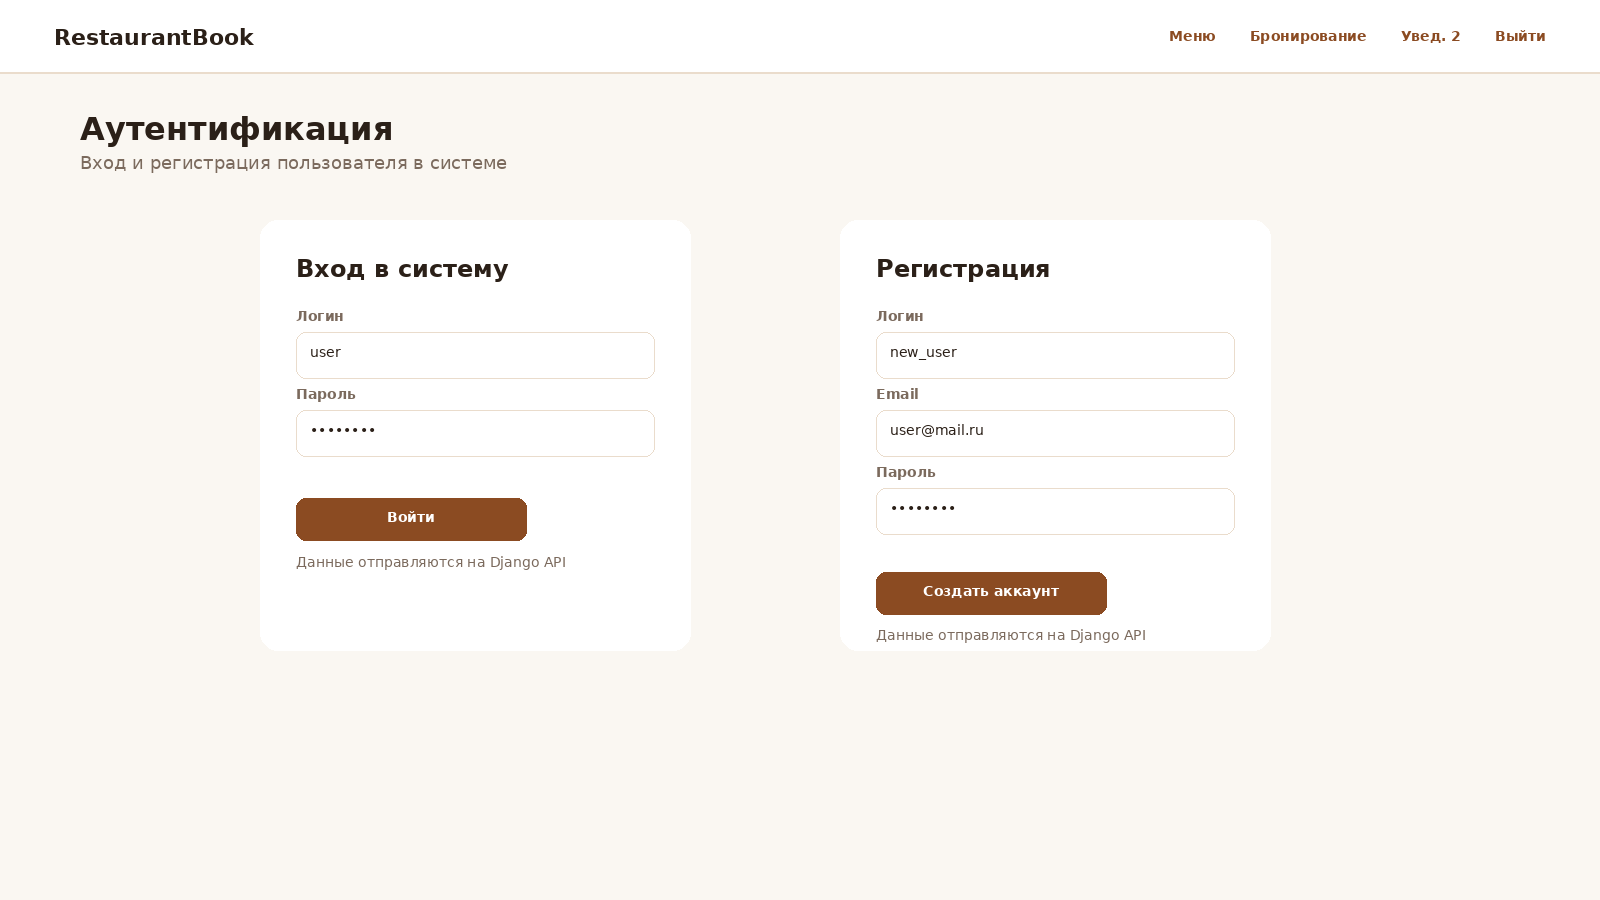
\includegraphics[width=0.82\textwidth]{wf_auth}
    \caption{Пользовательский шаблон страниц входа и регистрации}
    \label{fig:wf_auth}
\end{figure}

На рисунке~\ref{fig:wf_menu} представлен шаблон страницы меню ресторана.
На странице показаны категории блюд, карточки с названием, описанием,
ценой и изображением. Изображения блюд загружаются через административный
CRUD-интерфейс и отображаются пользователю в меню.

\begin{figure}[H]
    \centering
    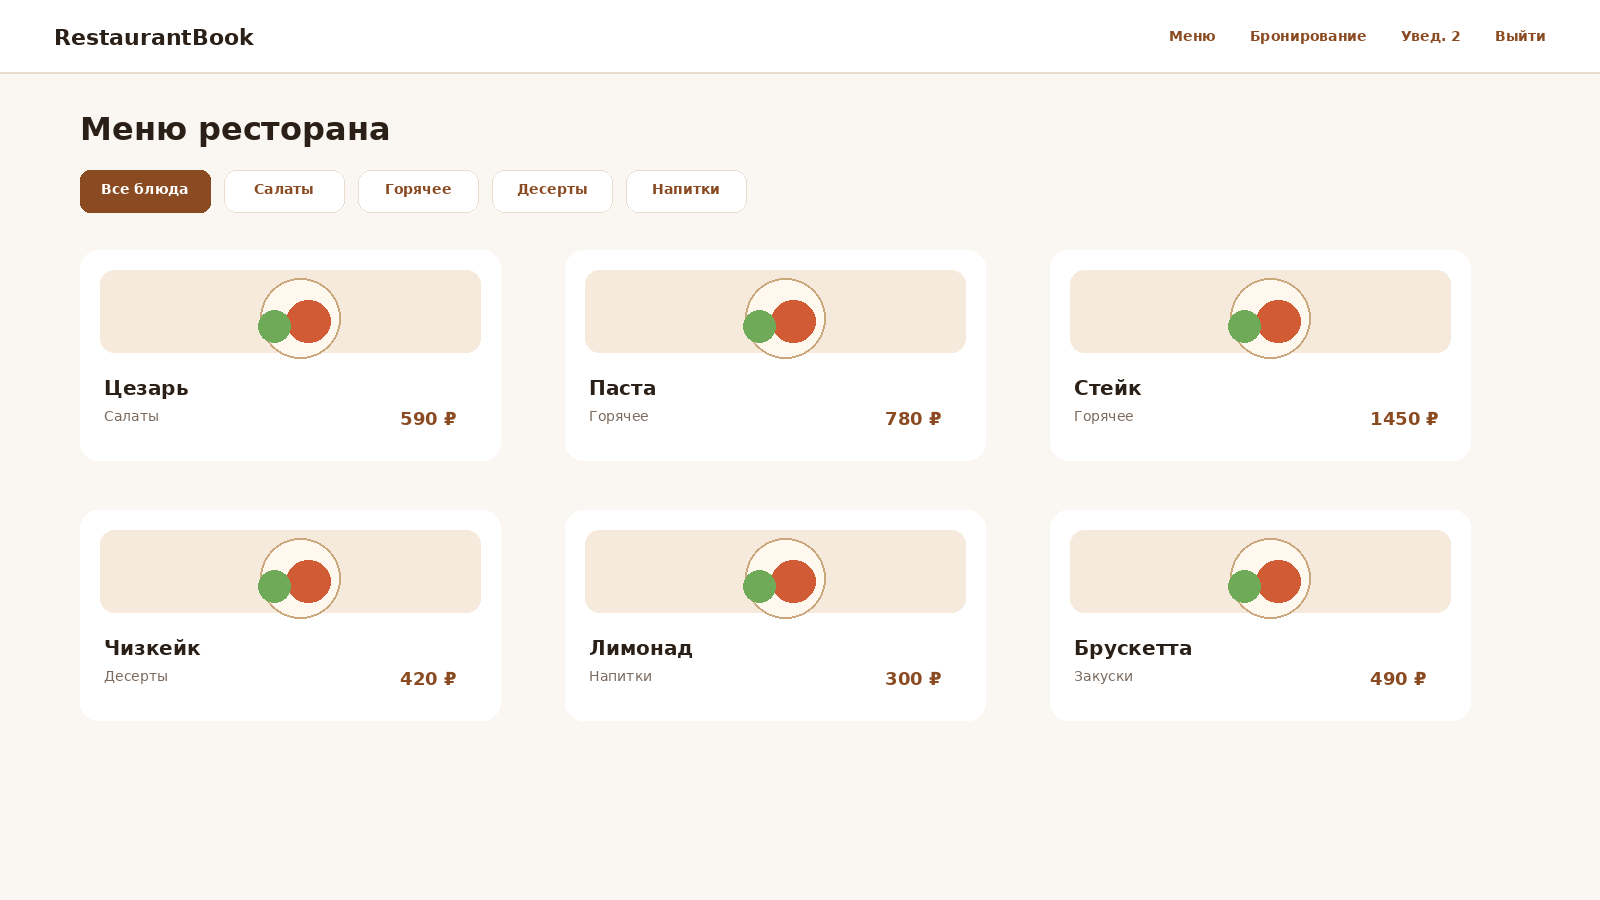
\includegraphics[width=0.95\textwidth]{wf_menu}
    \caption{Пользовательский шаблон страницы меню ресторана}
    \label{fig:wf_menu}
\end{figure}

На рисунке~\ref{fig:wf_booking} представлен шаблон страницы бронирования.
Пользователь выбирает дату, время начала и окончания, количество гостей и
столик. На основе этих данных система проверяет доступность столика и
создаёт бронирование только при отсутствии пересечений по времени. В
шаблоне также предусмотрено информационное сообщение о доступности
выбранного столика для указанного интервала, а после создания заявки
пользователь получает внутреннее уведомление и email-подтверждение.

\begin{figure}[H]
    \centering
    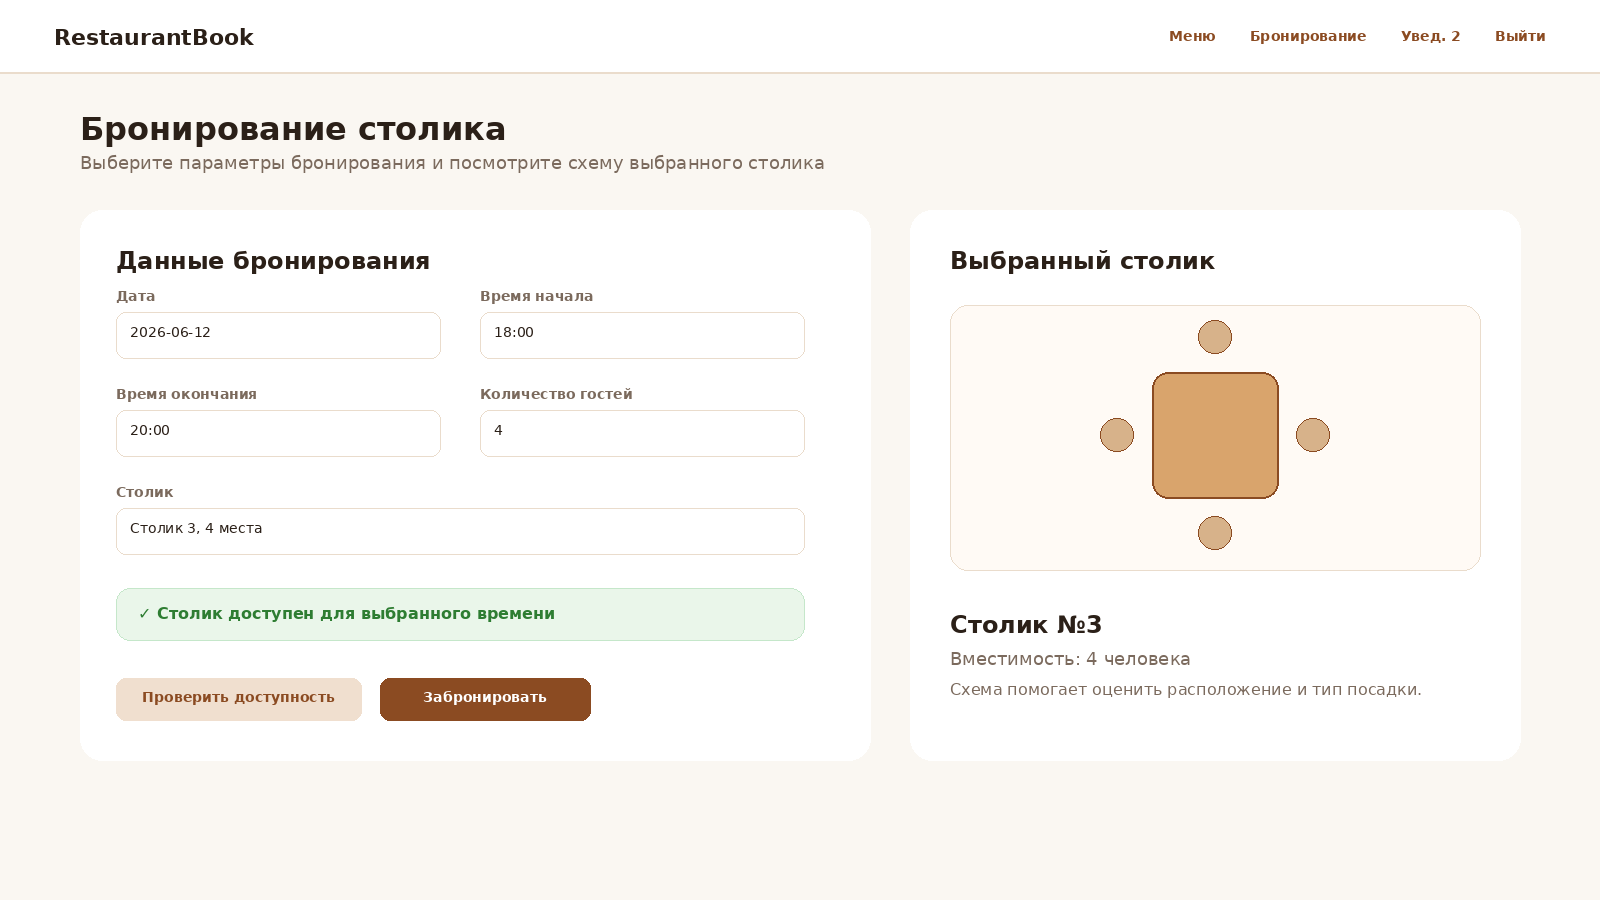
\includegraphics[width=0.95\textwidth]{wf_booking}
    \caption{Пользовательский шаблон страницы бронирования столика}
    \label{fig:wf_booking}
\end{figure}

На рисунке~\ref{fig:wf_notifications} представлен шаблон страницы
уведомлений. Пользователь видит уведомления о создании, подтверждении,
напоминании и отмене бронирования. В тексте уведомления предусмотрено
сообщение о PDF-подтверждении, отправленном на почту. Email-рассылка
дублирует наиболее важные уведомления: подтверждение бронирования,
напоминание, отмену или изменение статуса.

\begin{figure}[H]
    \centering
    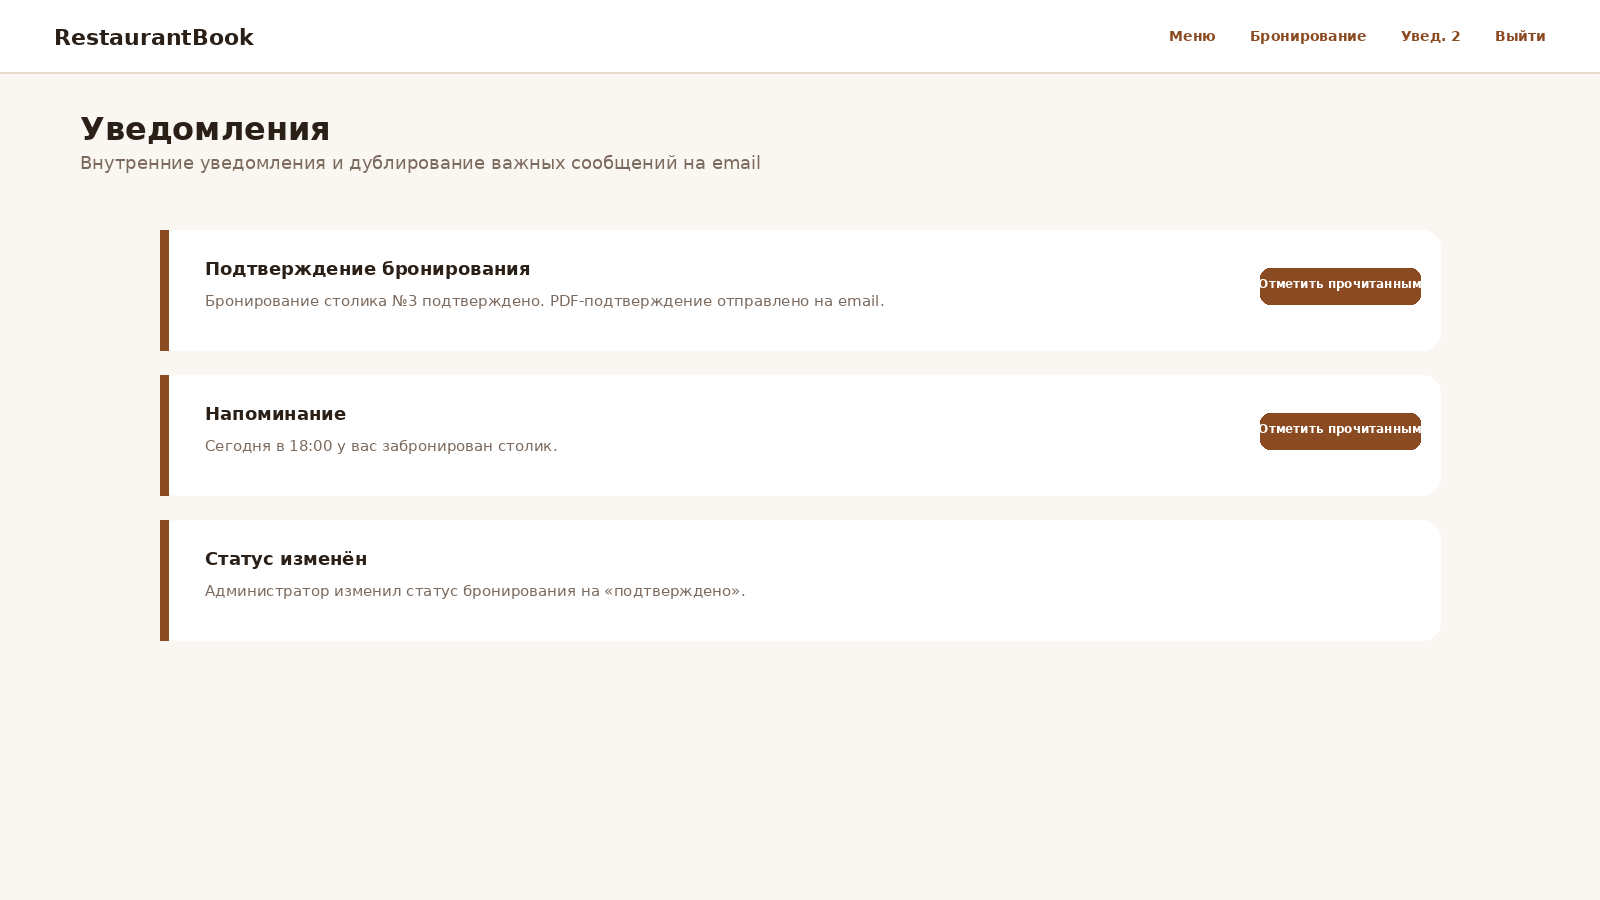
\includegraphics[width=0.82\textwidth]{wf_notifications}
    \caption{Пользовательский шаблон страницы уведомлений}
    \label{fig:wf_notifications}
\end{figure}

\subsubsection*{Административные шаблоны}
\addcontentsline{toc}{subsubsection}{Административные шаблоны}

На рисунке~\ref{fig:wf_admin} представлен шаблон административной панели
бронирований. Администратор фильтрует заявки по дате, столику и статусу,
видит время бронирования, изменяет или удаляет записи, а также
экспортирует данные в CSV и PDF.

\begin{figure}[H]
    \centering
    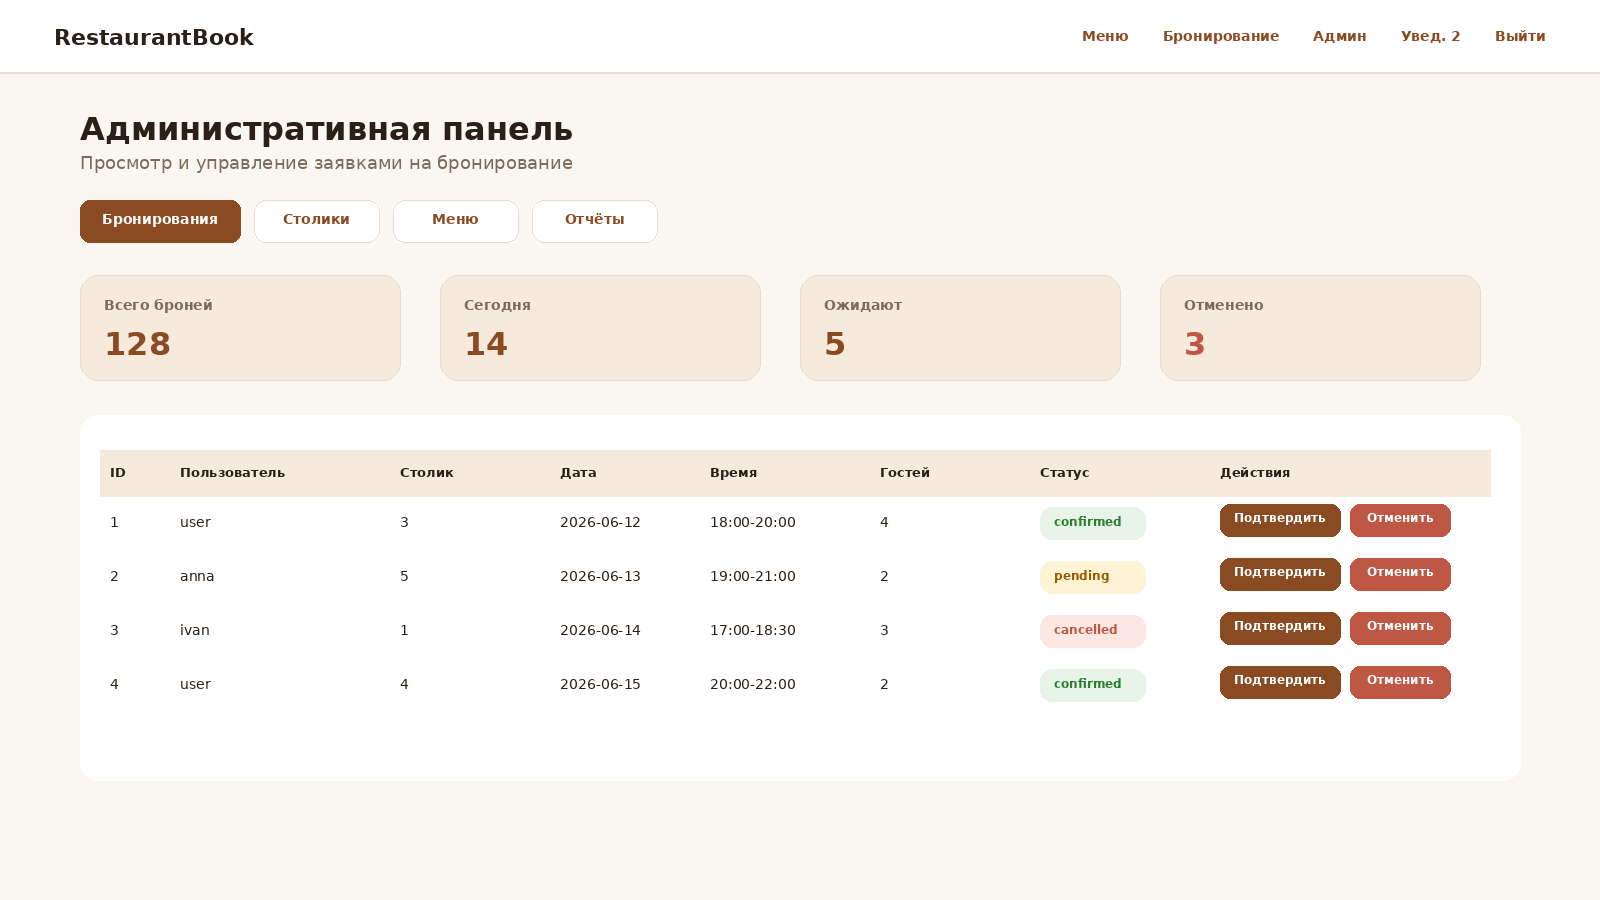
\includegraphics[width=0.95\textwidth]{wf_admin}
    \caption{Административный шаблон управления бронированиями}
    \label{fig:wf_admin}
\end{figure}

\newpage
На рисунке~\ref{fig:wf_crud} представлен шаблон административного
раздела управления столиками и меню. В интерфейсе предусмотрены
добавление, редактирование и удаление записей, переключение между
вкладками «Столики» и «Меню», а также загрузка фотографии столика и
изображения позиции меню.

\begin{figure}[H]
    \centering
    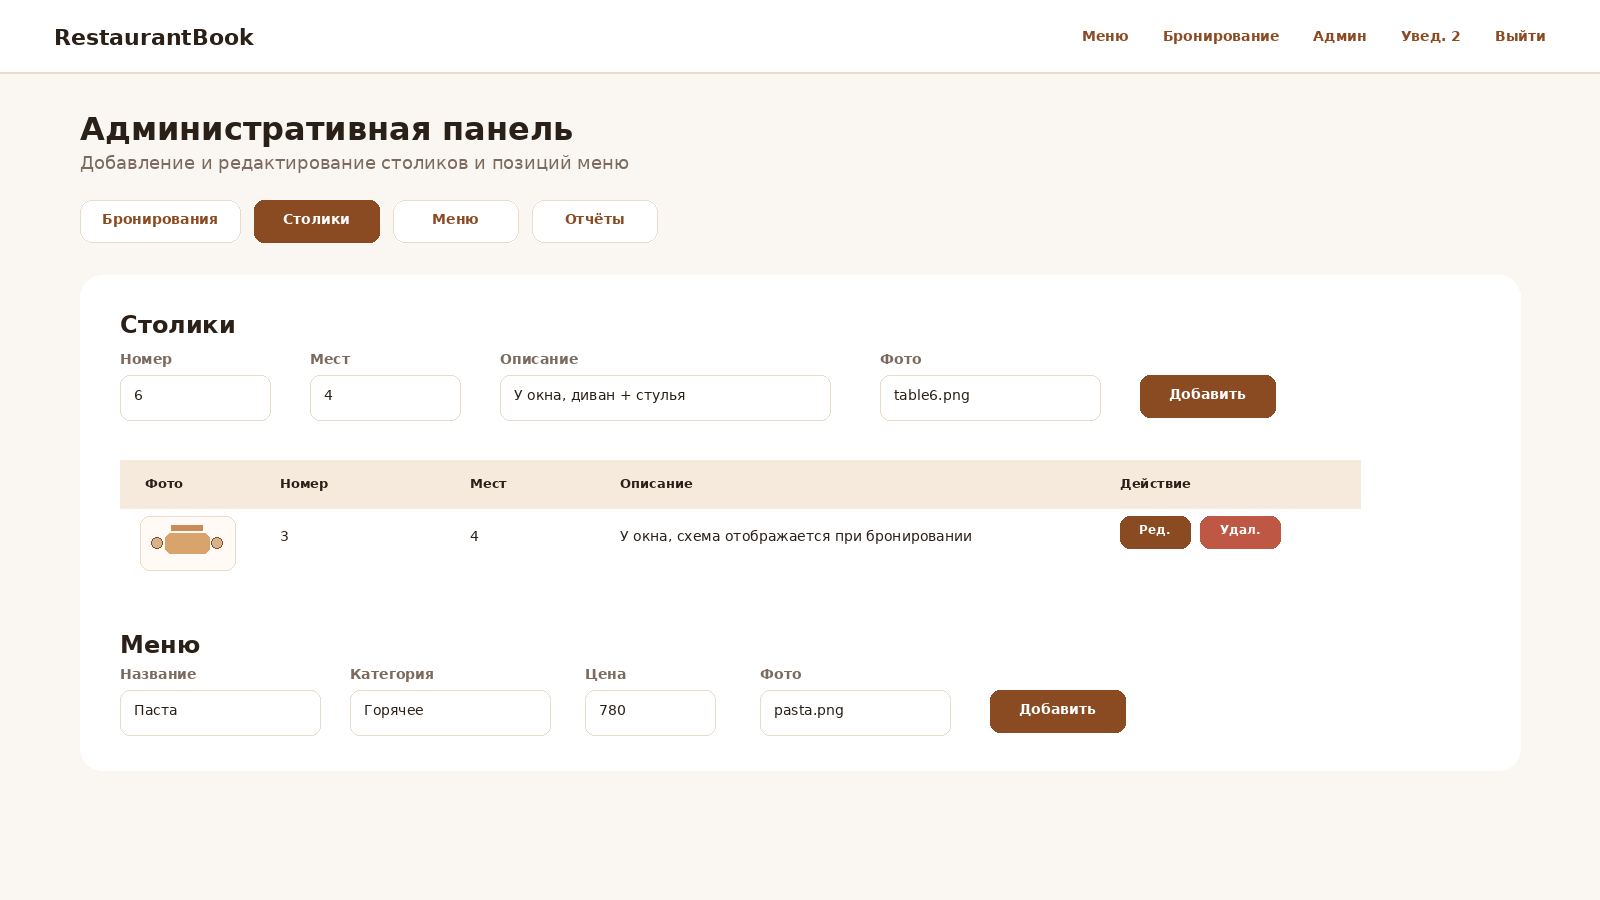
\includegraphics[width=0.90\textwidth]{wf_crud}
    \caption{Административный шаблон управления столиками и меню}
    \label{fig:wf_crud}
\end{figure}

\newpage
На рисунке~\ref{fig:wf_reports} представлен шаблон страницы отчётов и
аналитики. В интерфейсе предусмотрены показатели общего количества
бронирований, бронирований за месяц, загруженности и отменённых заявок,
фильтры по периоду, столику и статусу, а также кнопки скачивания CSV и
PDF.

\begin{figure}[H]
    \centering
    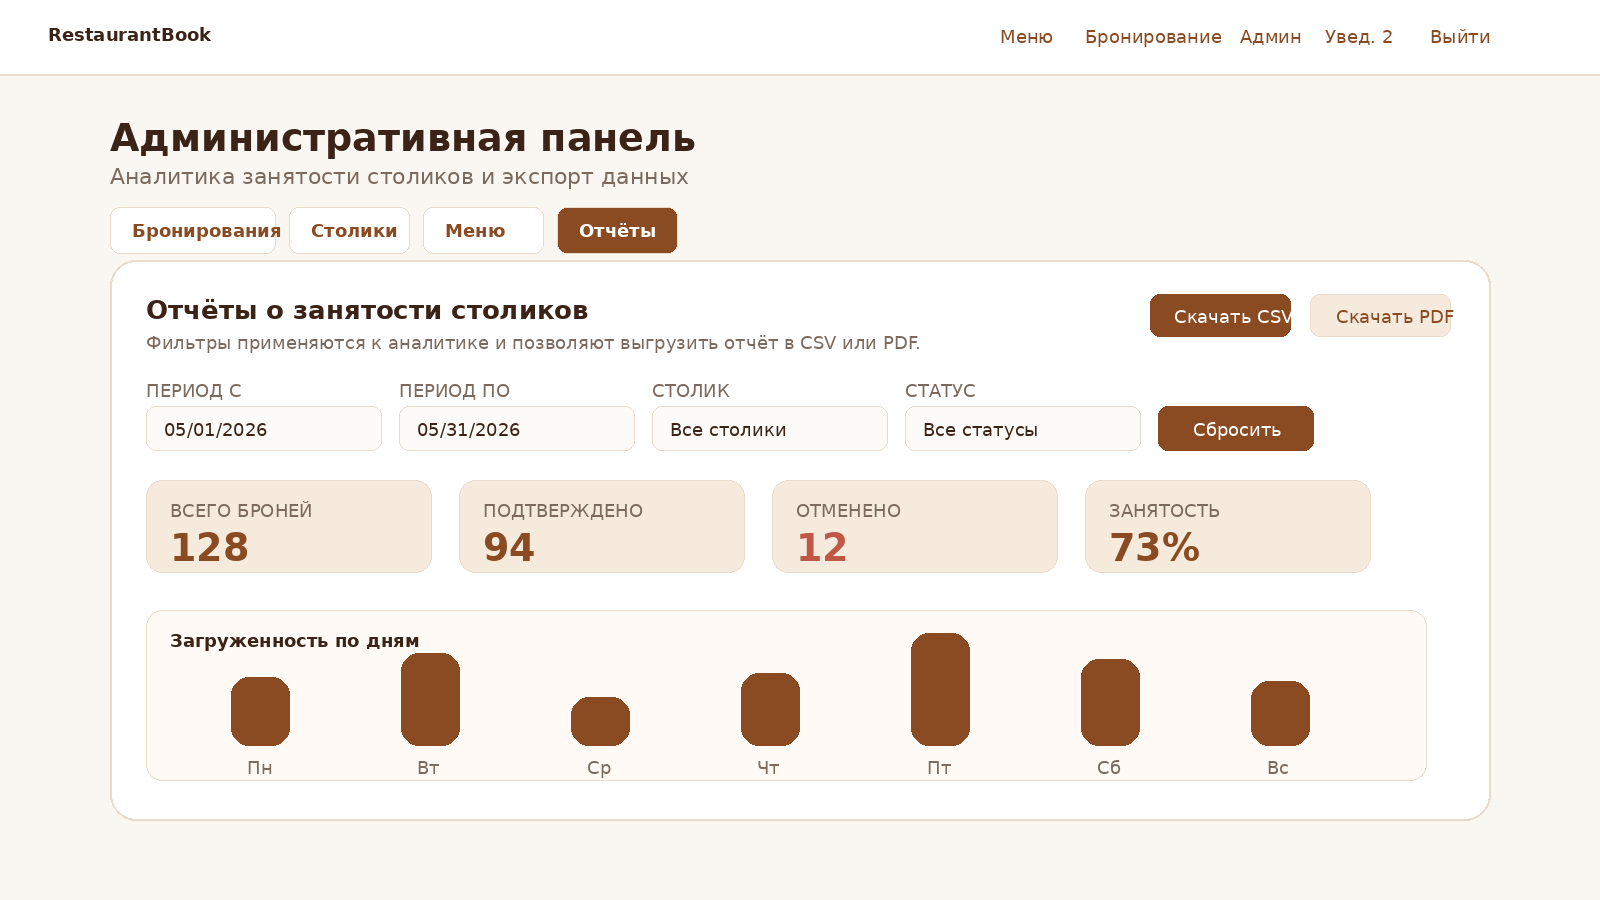
\includegraphics[width=0.90\textwidth]{wf_reports}
    \caption{Административный шаблон отчётов и аналитики}
    \label{fig:wf_reports}
\end{figure}

Таким образом, во второй главе отражены основные проектные решения:
роли пользователей, функциональные требования, варианты использования,
структура базы данных, проверка доступности столиков, внутренние
уведомления, email-рассылка, PDF-подтверждения и шаблоны ключевых страниц. Пользовательские шаблоны
показывают сценарии регистрации, просмотра меню, бронирования и
получения уведомлений, а административные шаблоны --- управление
столиками, меню, бронированиями и отчётностью.
